\chapter{Model training and device classification results} \label{chap6}

In the previous chapters we described how to create a Neural Network classifier able to solve the device identification task and how to obtain and preprocess a dataset to train the classifier on. In this chapter we present and discuss the results of the training of the classifier models on the two proposed dataset alongside with an evaluation of their performances.

As said before, the results presented in this chapter are obtained after dividing the datasets in three subsets: the training set over which the classifier are trained, the validation set, used to monitor the performances during the training and the test set, used to evaluate the real performances of the classifiers.

In section \secref{res_lb} we discuss the choice of the architecture depending on the lookback value $L$ and how the choice of the latter can impact the training of the selected architecture. In \secref{res_test} we will then recall the main features of the selected architectures and show the results of the classifiers training, alongside with their final performances. Finally in \secref{res_unseen} we will presents the results of the implementation of the trained classifier for the identification of devices not included in the original dataset. All the computations have been performed on a machine with a Ryzen 6 core CPU, an NVIDIA GTX 1660 Super GPU and 32GB of memory.


\section{Classifier architecture and time series length}\label{res_lb}

In \chapref{chap4} we presented the statistic and class division of the 4SICS and IoT Sentinel dataset, respectively in \tabref{tab:4sicsdev} and \tabref{tab:iotdev}. During the preprocessing operation the 4SICS dataset timeseries were created using a value of the lookback, defined in \secref{fig:ts_processing}, of $L=100$. The IoT dataset on the other hand was preprocessed using a value of $L=30$. As previously stated the choice of using a smaller lookback value is made in order to maximize the number of obtained timeseries and, consequently, the dataset dimension, with the goal of maximizing the final performance of the model. 

This choice however is not compatible with the use of the 1B\_AP architecture, namely the general proposed model, so the 1B\_NP architecture should be used instead. The reason for the incompatibility of the 1B\_AP architecture with a value $L=30$ is the presence of the pooling layers. 
Even when using a poolsize of 2, the smallest possible value, each layer halves the size of the vector. This fact, combined with the size reduction caused by the filters\footnote{In the 1B\_AP architecture the zero padding technique is not implemented since we want to reduce the input dimensionality. Indicating with $K$ the size of the filter, after a convolutional layers the size of the input and output vector will the differ by $K-1$.}, results in a too low final dimension of the input or, in some cases, even in the mathematical incompatibility of the operations.

The chosen value of $L=30$ corresponds to the lowest value for which the training performance of the model is not critically affected. This value was estimated training several 1B\_NP classifiers using samples obtained from the dataset preprocessing with different values of $L$. The dataset used for this estimation is the 4SICS dataset, in order to avoid possible biases caused by the training dataset size. 
In \figref{fig:res_lb_val} the loss function and model accuracy, for different lookback values, over the training and validation dataset is shown. As we can see from these plots  using values of $L=10,20$ results in divergence of the training and validation loss function. This behaviour indicates the presence of overfitting during the training. This may be explained considering that, for low $L$ valus some variety is lost in the time series, resulting in a too high model complexity for the provided input dimension.

The classifier trained with $L=30$ on the other hand does not present such behaviour, justifying the choice made for the lookback value for this architecture. Additional plots of the loss function and model accuracy for higher values of the lookback are shown in \appref{app:lb_bonus_res}.


\begin{figure}[!h]
    \centering
    \begin{minipage}[c]{0.49\textwidth}
        \vspace{0pt}
        \centering
        \subfloat[Loss function with lookback $L=10$]{
        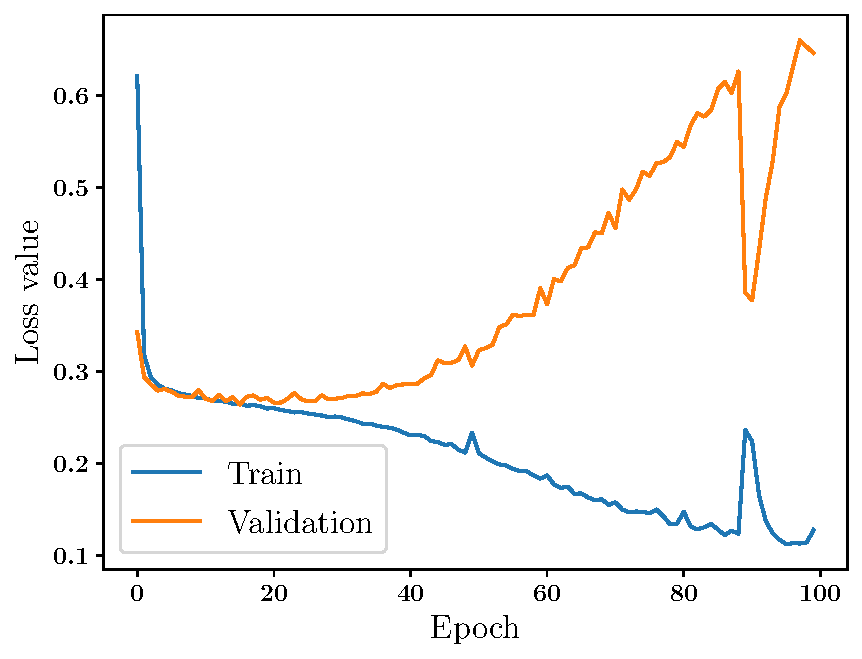
\includegraphics[width=\textwidth]{images/results/LB_test_10_20210613-180735__type_1branch_no_pool__st_scale_sub__lb_10__act_elu__nf_16__ks_10__nn_50__l2_1e-05__bs_200__ep_100__loss.pdf}
            \label{fig:lb_10_loss}
        }
    \end{minipage}%
    \hfill%
    \begin{minipage}[c]{0.49\textwidth}
        \vspace{0pt}
        \centering
        \subfloat[Accuracy with lookback $L=10$]{
        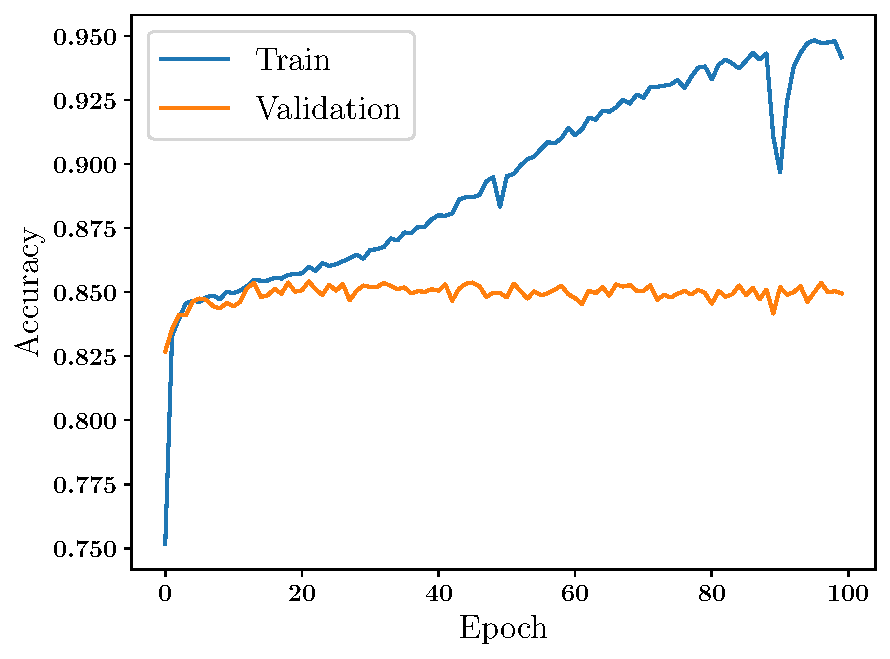
\includegraphics[width=\textwidth]{images/results/LB_test_10_20210613-180735__type_1branch_no_pool__st_scale_sub__lb_10__act_elu__nf_16__ks_10__nn_50__l2_1e-05__bs_200__ep_100___accuracy.pdf}
            \label{fig:lb_10_acc}
        }
    \end{minipage}
        \begin{minipage}[c]{0.49\textwidth}
        \vspace{0pt}
        \centering
        \subfloat[Loss function with lookback $L=20$]{
        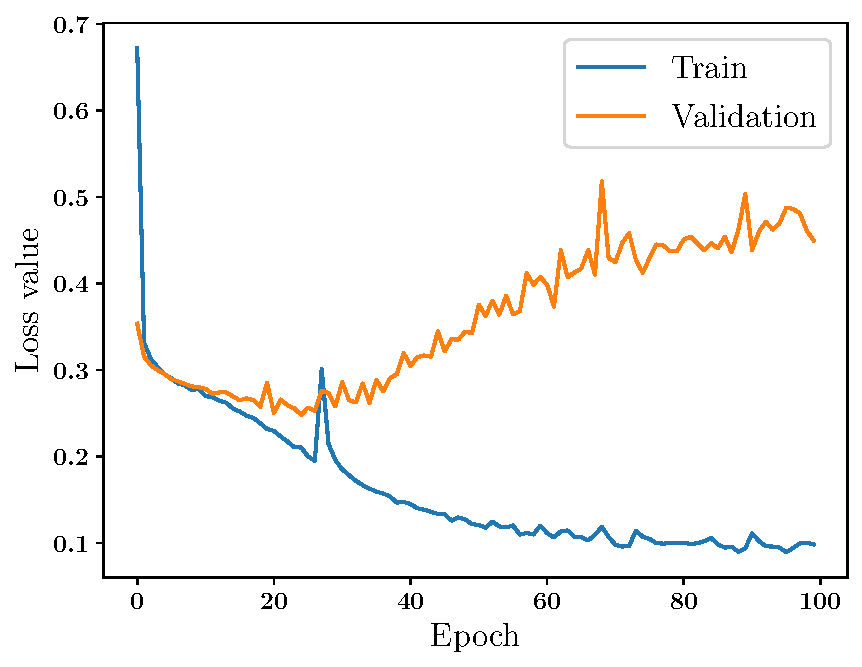
\includegraphics[width=\textwidth]{images/results/LB_test_20_20210613-180946__type_1branch_no_pool__st_scale_sub__lb_20__act_elu__nf_16__ks_10__nn_50__l2_1e-05__bs_200__ep_100__loss.pdf}
            \label{fig:lb_20_loss}
        }
    \end{minipage}%
    \hfill%
    \begin{minipage}[c]{0.49\textwidth}
        \vspace{0pt}
        \centering
        \subfloat[Accuracy with lookback $L=20$]{
        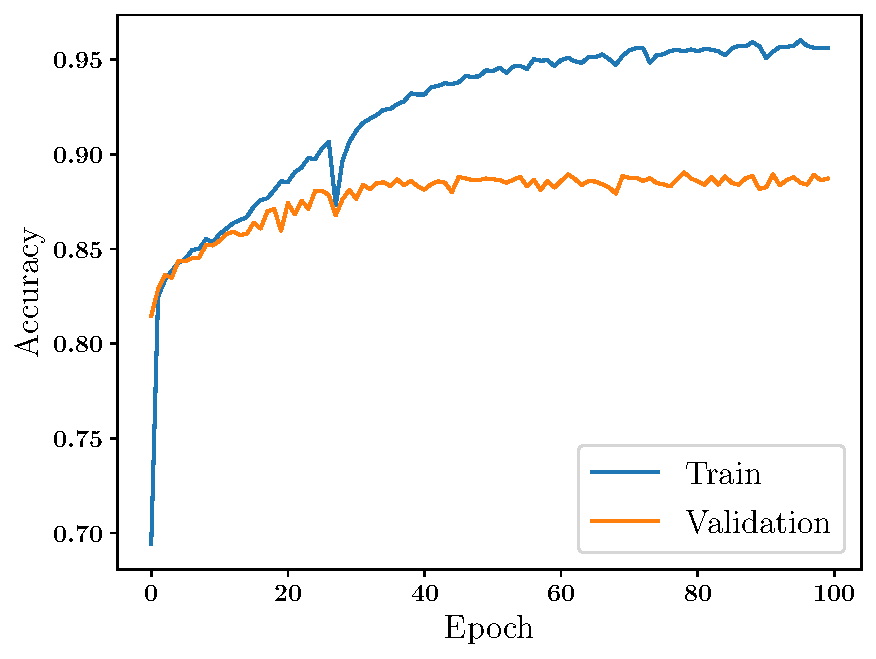
\includegraphics[width=\textwidth]{images/results/LB_test_20_20210613-180946__type_1branch_no_pool__st_scale_sub__lb_20__act_elu__nf_16__ks_10__nn_50__l2_1e-05__bs_200__ep_100___accuracy.pdf}
            \label{fig:lb_20_acc}
        }
    \end{minipage}    \begin{minipage}[c]{0.49\textwidth}
        \vspace{0pt}
        \centering
        \subfloat[Loss function with lookback $L=30$]{
        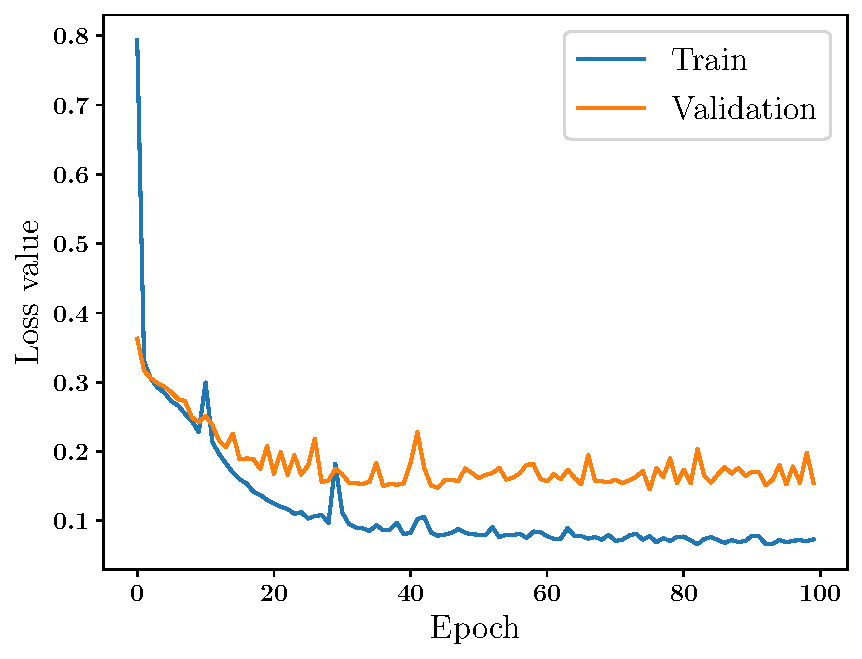
\includegraphics[width=\textwidth]{images/results/LB_test_30_20210613-181249__type_1branch_no_pool__st_scale_sub__lb_30__act_elu__nf_16__ks_10__nn_50__l2_1e-05__bs_200__ep_100__loss.pdf}
            \label{fig:lb_30_loss}
        }
    \end{minipage}%
    \hfill%
    \begin{minipage}[c]{0.49\textwidth}
        \vspace{0pt}
        \centering
        \subfloat[Accuracy with lookback $L=30$]{
        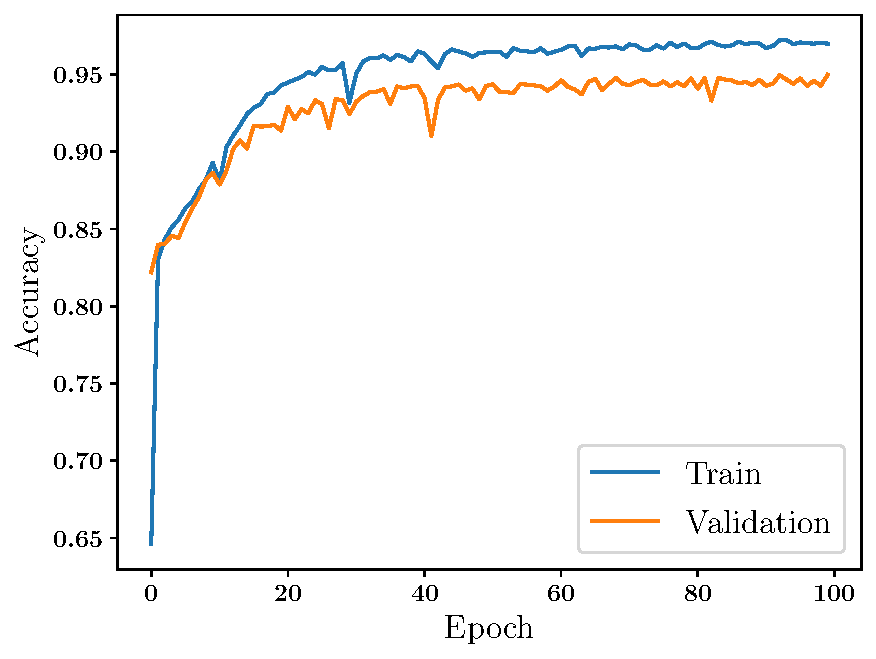
\includegraphics[width=\textwidth]{images/results/LB_test_30_20210613-181249__type_1branch_no_pool__st_scale_sub__lb_30__act_elu__nf_16__ks_10__nn_50__l2_1e-05__bs_200__ep_100___accuracy.pdf}
            \label{fig:lb_30_acc}
        }
    \end{minipage}


    \caption{lookback analysis}
    \label{fig:res_lb_val}
\end{figure}





\section{Model training and final performance}\label{res_test}

In this section we present the architecture and final performances of the proposed classifiers, after the training procedure, for both datasets. The performances have been evaluated using the test sets and the possible presence of over or under fitting behaviour is monitored, as shown previously, using the validation set. 

As previously said, the different size of the two dataset imposed the led to the choice of implementing the 1B\_NP architecture, for the classification of the IoT dataset devices while, for the 4SICS dataset device classification, the 1B\_AP architecture was implemented. 
In \tabref{tab:final_models} we recall the main features of the two architectures, alongside with the chose value of the hyperparameters introduced in \chapref{chap5}.

The behaviour of these models during the training, alongside with the final classification accuracy reached, is discussed in \secref{4sics_final_res} and \secref{iot_final_res} respectively for the 4SICS and IoT dataset.


%As previously said, for the 4SICS dataset, the 1B\_AP architecture was used while, for the %IoT dataset, the 1B\_NP one was implemented. Before showing the final results, in the %following list, we recall the main features and reported the chosen hyperparameters of these %classifier models:
%\begin{itemize}
%    \item Each convolutional layer contains 16 filters of size 10
%    \item Zero padding technique implementation in the 1B\_NP architecture
%    \item Pooling layers, if present, have pool size 2
%    \item ELU activation function and L2 regularization are implemented in each layer
%    \item Dropout rate of 30\% 
%    \item The first layer after the concatenation features 50 neurons, following layers have %each half neurons of the previous one
%    \item Adam optimizer and Categorical Crossentropy loss function
%\end{itemize}


%As previously said, for the 4SICS dataset, the 1B\_AP architecture was used while, for the %IoT dataset, the 1B\_NP one was implemented. Before showing the final results, we ropert n %\tabref{tab:final_models} the main features and the chosen hyperparameters of the used %classifier.

\begin{table}[h]
    \centering
    \begin{tabular}{lccm{5cm}}
    \Xhline{3\arrayrulewidth} 
       \multirow{2}{*}{\textbf{Parameter}}   &
       \multicolumn{2}{c}{\textbf{Dataset}} & \multirow{2}{*}{\textbf{Description}}\\
        & \textbf{4SICS dataset} & \textbf{IoT dataset} & 
       \\
    \Xhline{2\arrayrulewidth} 
        Architecture  & 1B\_AP & 1B\_NP & \footnotesize{Classifier architecture chosen from the ones shown in \chapref{chap5}}\\ \hline
        Filter number &\multicolumn{2}{c}{16} & \footnotesize{Number of filter contained in each convolutional layer} \\ \hline
        Filter dimension &\multicolumn{2}{c}{10} & \footnotesize{Dimension of the convolutional layer filters }\\ \hline
        Pool size  & 2 & $\boldsymbol{-}$ & \footnotesize{Pool dimension in pooling layers}\\ \hline
        Dropout Rate  &\multicolumn{2}{c}{30\%} &\footnotesize{ Probability of excluding a neuron in a dense layer}\\ \hline
        Number of neurons  & \multicolumn{2}{c}{50} & \footnotesize{Neurons in the first dense layer after concatenation }\\ \hline
        Optimizer    &\multicolumn{2}{c}{Adam} & \footnotesize{Optimization algorithm used to update the free parameters} \\ \hline
        Loss function  & \multicolumn{2}{c}{Categorical Crossentropy} & \footnotesize{Function to minimize during the training}\\ \hline
        Hidden layers activation & \multicolumn{2}{c}{ELU} & \footnotesize{Function applied to the output of each hidden layer} \\ \hline
        Final layers activation & \multicolumn{2}{c}{Softmax} & \footnotesize{Function applied to the final output of the classifier} \\ 
    \Xhline{3\arrayrulewidth}
    \end{tabular}
    \caption{Features and selected hyperparameters of the final classifier models. The results of the training and the final performance evaluation of these models are shown in \secref{4sics_final_res} and \secref{iot_final_res} respectively for the 4SICS and IoT dataset.}
    \label{tab:final_models}
\end{table}



\subsection{4SICS dataset}
\label{4sics_final_res}

The 1B\_AP model is trained using the samples, reported in \tabref{tab:4sicsdev}, obtained from the preprocess of the 4SICS dataset with a lookback value of $L=100$. The training is performed for 300 epochs using a batch size\footnote{The batch size indicates the number to use in the computation of the loss function during the training before updating the free parameters of the selected classifier.} of 200. 

In \figref{fig:4sics_results} the loss function and of the model accuracy evolution, for both the training and validation set, is show. As we can see the model is able to reach high performances and does not show overfitting behaviour. 

After the training the final accuracy of the model is evaluated using the set, by comparing the predicted class of the devices with their true class. This comparison is done using a confusion matrix, shown in \figref{fig:4sics_results_cm}.\\
As we can see for all classes more than 90\% of the predicted labels are correct, with the Switch and Router class having 100\% correct predictions. From this matrix we also estimate a 96.2\% overall test accuracy.

\begin{figure}[!h]
    \centering
    \begin{minipage}[c]{0.49\linewidth}
        \vspace{0pt}
        \centering
        \subfloat[Loss function during training]{
        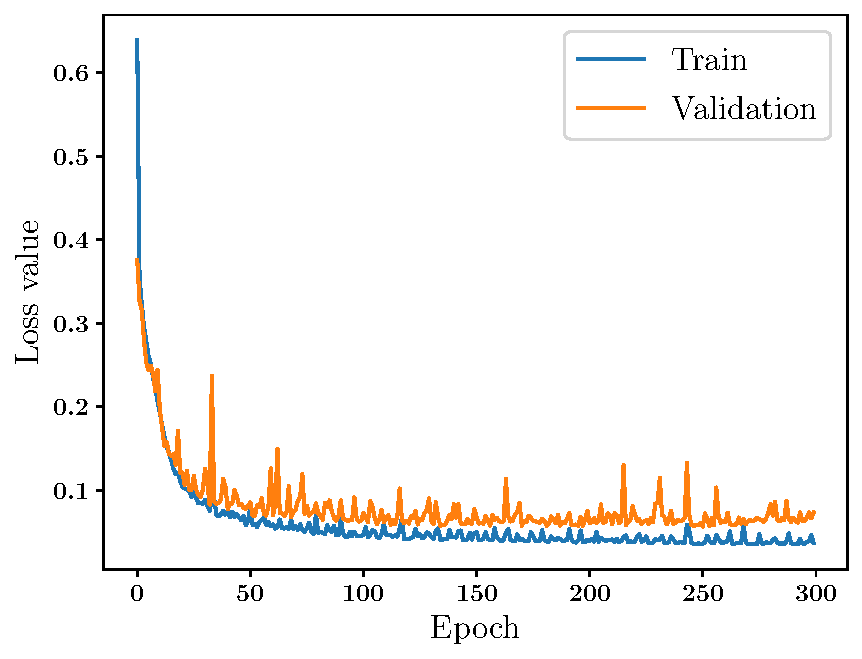
\includegraphics[width=\textwidth]{images/results/4SICS_clasf_20210613-174409__type_1branch__st_scale_sub__lb_100__act_elu__nf_16__ks_10__nn_50__l2_1e-05__bs_200__ep_300__loss.pdf}
            \label{fig:4sics_loss}
        }
    \end{minipage}%
    \hfill%
    \begin{minipage}[c]{0.49\linewidth}
        \vspace{0pt}
        \centering
        \subfloat[Accuracy during training]{  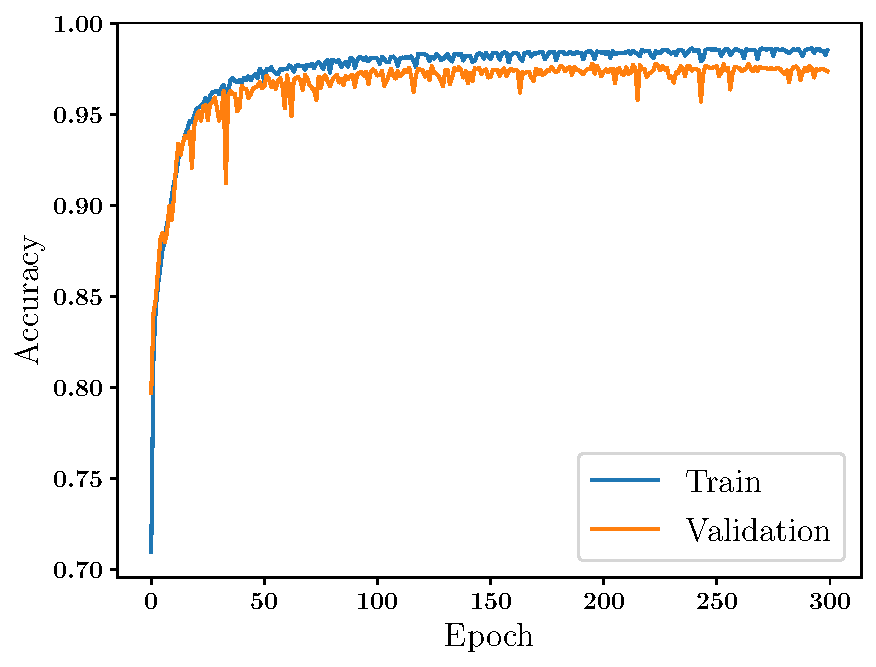
\includegraphics[width=\textwidth]{images/results/4SICS_clasf_20210613-174409__type_1branch__st_scale_sub__lb_100__act_elu__nf_16__ks_10__nn_50__l2_1e-05__bs_200__ep_300___accuracy.pdf}
        \label{fig:4sics_loss}
        }
    \end{minipage}%
    \caption{Model accuracy and loss function during training over both training and validation set. Results obtained during the training of the  1B\_AP architecture over the 4SICS dataset. }
    \label{fig:4sics_results}
\end{figure}


%
%\begin{figure}[h]
%    \centering
%        \includegraphics[width=0.6\textwidth]{images/results/4SICS_clasf_20210613-174409__typ%e_1branch__st_scale_sub__lb_100__act_elu__nf_16__ks_10__nn_50__l2_1e-05__bs_200__ep_3%00___cm.pdf}
%    \caption{Final 1B\_AP classifier predictions on 4SICS test set. Predictions are %visualized using a confusion matrix.  The colormap represents the fraction of samples %belonging to a certain prediction class.}
%    \label{fig:4sics_results_cm}
%\end{figure}


\begin{figure}[!h]
\begin{minipage}{0.6\linewidth}
    \centering
        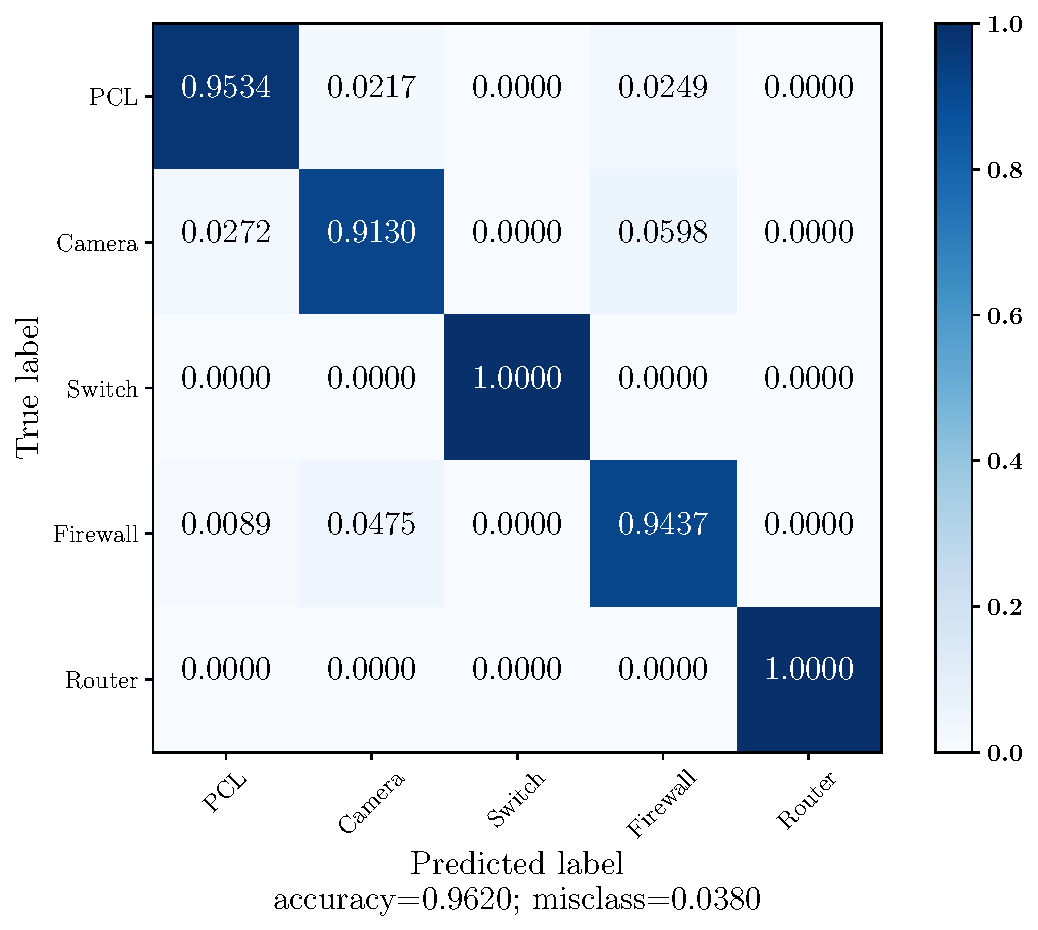
\includegraphics[width=\textwidth]{images/results/4SICS_clasf_20210613-174409__type_1branch__st_scale_sub__lb_100__act_elu__nf_16__ks_10__nn_50__l2_1e-05__bs_200__ep_300___cm.pdf}
\end{minipage}
\hfill
\begin{minipage}{0.29\linewidth}
\caption{Final 1B\_AP classifier predictions on 4SICS test set. Predictions are visualized using a confusion matrix.  The colormap represents the fraction of samples belonging to a certain prediction class.}
     \label{fig:4sics_results_cm}
\end{minipage}
\end{figure}



\subsection{IoT dataset}
\label{iot_final_res}


The 1B\_NP model is trained using the samples, reported in \tabref{tab:iotdev}, obtained from the preprocess of the IoT dataset with a lookback value of $L=30$. 

The training is performed for 300 epochs using a batch size of 100. 
In \figref{fig:iot_results} the loss function and of the model accuracy evolution, for both the training and validation set, is show. Like for the previous case, also this model is able to reach high performances and does not show overfitting behaviour. 
As for the previous model we evaluate the final model accuracy using a confusion matrix, shown in \figref{fig:iot_results_cm}. In this case we observe a test accuracy higher than 95\%, for all the device classes, with an estimated overall test accuracy of 98.6\%
This result does also validate the chosen lookback value $L$ and architecture.

%As stated previously due to the small length of the timeseries the chosen architecture for %the device classification over the IoT Sentinel dataset in the 1B\_NP model, namely an %architecture with one convolutional "branch" without pooling layers. The selected device %classes, shown in \tabref{tab:iotdev}, have been preprocessed using a lookback $L=30$. The %training was performed for 300 epochs using a batch size of 100. 

%In \figref{fig:iot_results} the evolution of the loss function and of the model accuracy over %the training and validation set are shown. As for the previous dataset the model is able to %reach high performances and does not show overfitting behaviour, validating the choice of %architecture and lookback value. 
%

\begin{figure}[h]
    \centering
    \begin{minipage}[c]{0.49\linewidth}
        \vspace{0pt}
        \centering
        \subfloat[Loss function during training]{
        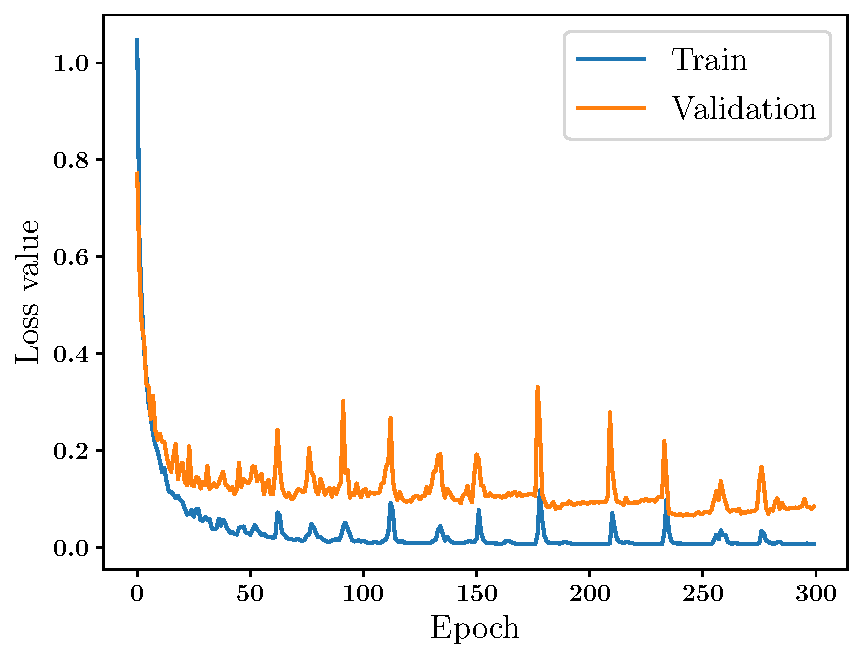
\includegraphics[width=\textwidth]{images/results/IoT_clasf_20210613-175027__type_1branch_no_pool__st_scale_sub__lb_30__act_elu__nf_16__ks_10__nn_50__l2_1e-05__bs_200__ep_300__loss.pdf}
            \label{fig:iot_loss}
        }
    \end{minipage}%
    \hfill%
    \begin{minipage}[c]{0.49\linewidth}
        \vspace{0pt}
        \centering
        \subfloat[Accuracy during training]{  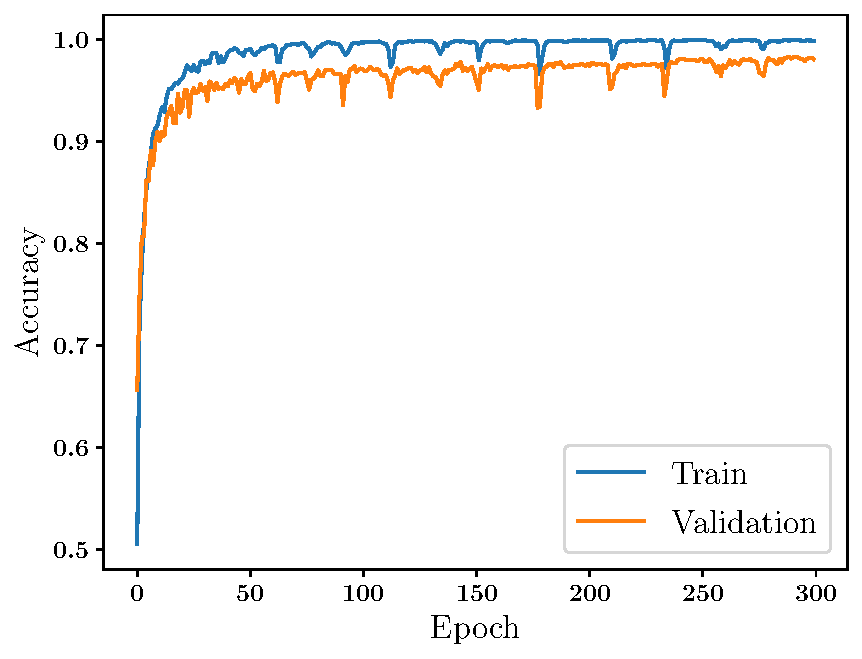
\includegraphics[width=\textwidth]{images/results/IoT_clasf_20210613-175027__type_1branch_no_pool__st_scale_sub__lb_30__act_elu__nf_16__ks_10__nn_50__l2_1e-05__bs_200__ep_300___accuracy.pdf}
        \label{fig:iot_loss}
        }
    \end{minipage}%
 \caption{Model accuracy and loss function during training over both training and validation set. Results obtained during the training of the  1B\_NP architecture over the IoT dataset. }       \label{fig:iot_results}
\end{figure}


%As for the previous model we evaluate the model performances using a confusion matrix, shown %in \figref{fig:4sics_results_cm}. For this dataset the classifier is able to reach a test %accuracy higher than 95\% for all the classes with an overall accurcay of 98.6\%

\begin{figure}[h]
\begin{minipage}{0.6\linewidth}
    \centering
        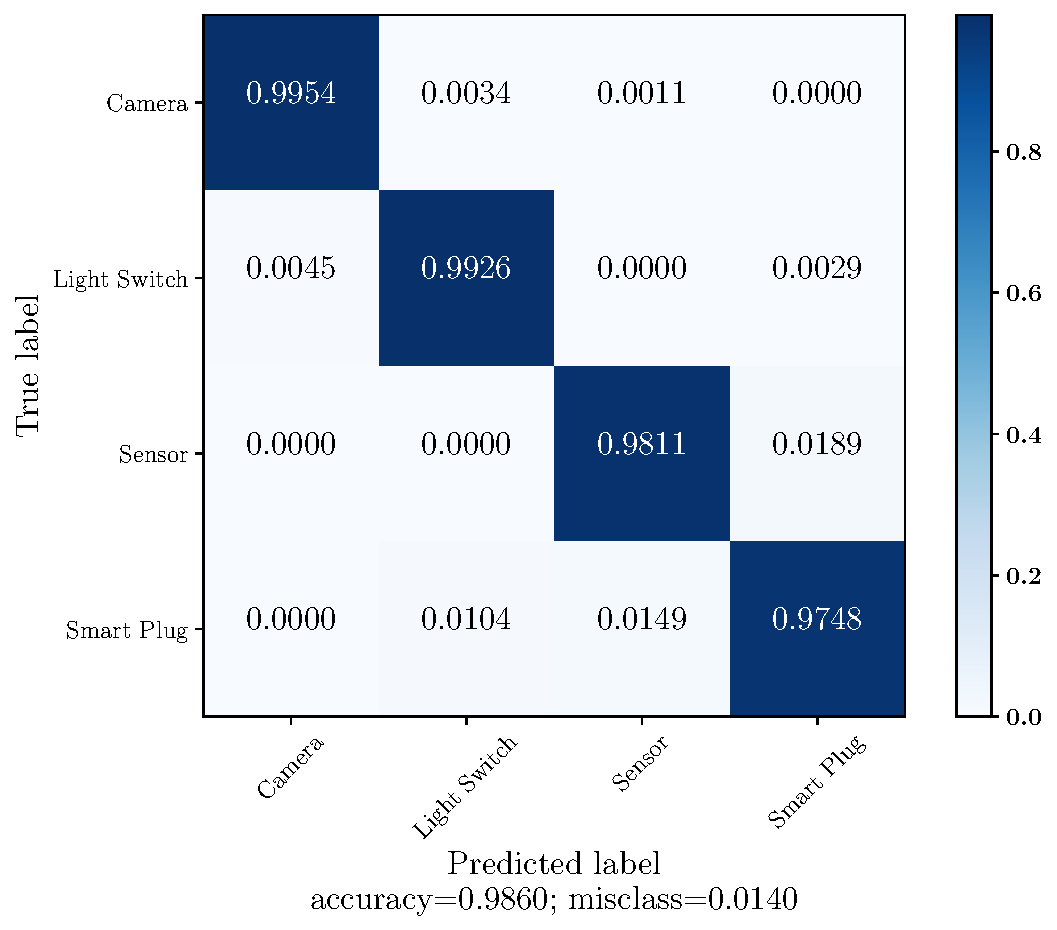
\includegraphics[width=\textwidth]{images/results/IoT_clasf_20210613-175027__type_1branch_no_pool__st_scale_sub__lb_30__act_elu__nf_16__ks_10__nn_50__l2_1e-05__bs_200__ep_300___cm.pdf}
\end{minipage}
\hfill
\begin{minipage}{0.29\linewidth}
  \caption{Final 1B\_NP classifier predictions on IoT Sentinel test set. Predictions are visualized using a confusion matrix.  The color map represents the fraction of samples belonging to a certain prediction class.} 
  \label{fig:iot_results_cm}
\end{minipage}
\end{figure}


\section{"Unseen" device classification}\label{res_unseen}

In the previous section we show that the proposed models are able, with great accuracy, of correctly of classifying a device. We now want to use the trained model in order to classify an "unseen" device.
More precisely our goal is to see if the classifier is able to recognize similarities between the device he was trained on and completely new devices. This test has is particularly interesting, due to how it translates in a real world application. In the real world in fact we can create more powerful classifiers, using deeper architecture or creating very big datasets with hundreds if not thousands of devices inside. The OT and IoT worlds however are continuously evolving and new devices are developed each year. The ability of the classifier of identifying a completely new device is then fundamental.

For each dataset we select two different devices, not included in the datasets described in \tabref{tab:4sicsdev} and \tabref{tab:iotdev}, but that belong to the device classes reported in them. We then processed their time series using exactly the same procedure and parameters as the one used to create the two training dataset. 
Once the new time series, with the respective communication protocol vector, are created, we use the trained classifiers to predict their device class. The final class prediction of the class of a device then corresponds to the class with the highest number of predicted time series. The result are shown as histograms in \figref{fig:4sics_unseen} and \figref{fig:iot_unseen} respectively for the 4SICS and IoT dataset. 



\begin{figure}[h]
    \centering
    \begin{minipage}[c]{0.49\linewidth}
        \vspace{0pt}
        \centering
        \subfloat[Class prediction of an "unseen" PLC]{
        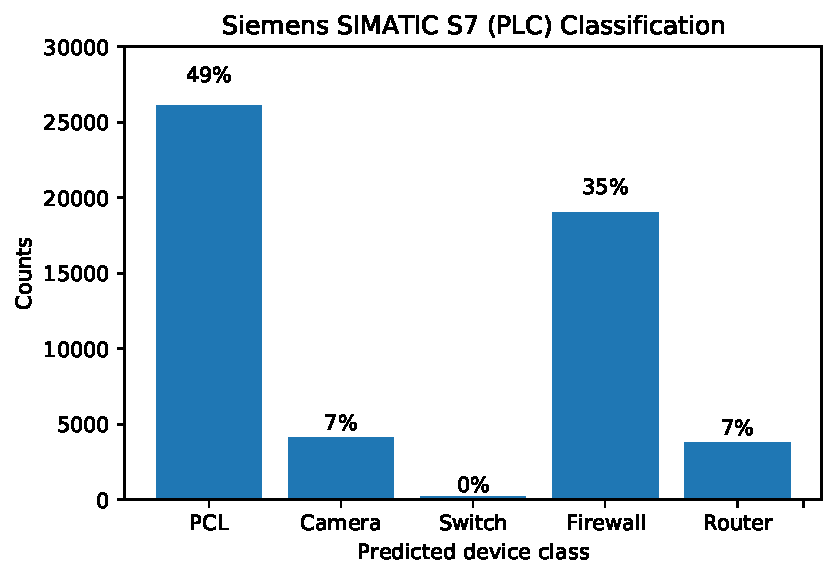
\includegraphics[width=\textwidth]{images/results/4sics_clasf_plc1_recognition.pdf}
            \label{fig:4sics_unseen_plc}
        }
    \end{minipage}%
    \hfill%
    \begin{minipage}[c]{0.49\linewidth}
        \vspace{0pt}
        \centering
        \subfloat[Class prediction of an "unseen" Router]
        {  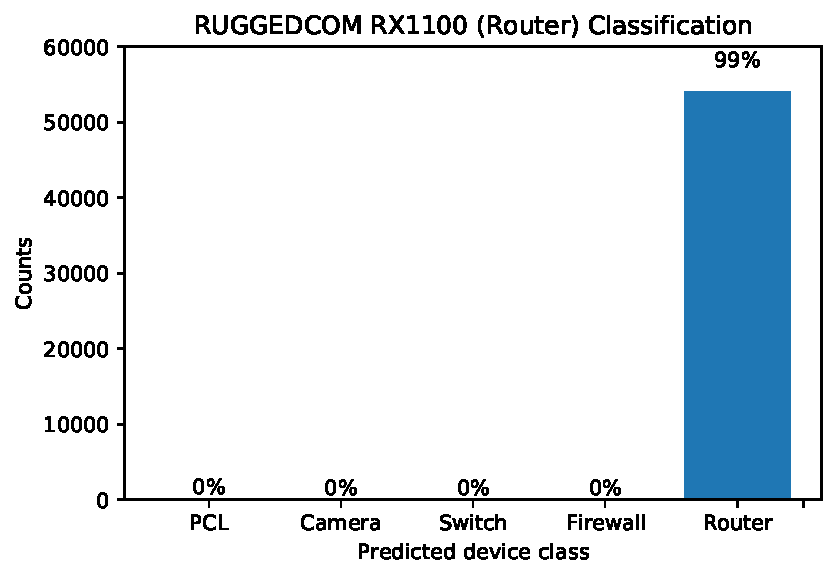
\includegraphics[width=\textwidth]{images/results/4sics_clasf_router_recognition.pdf}
            \label{fig:4sics_unseen_router}
        }
    \end{minipage}%
    \caption{Classification of "unseen" device using the trained 4SICS classifiers. Histogram shows the counts of time series assigned to each device class by the classifier. Selected devices belong to the PLC class, shown in \figref{fig:4sics_unseen_plc}, and Router class, shown in \figref{fig:4sics_unseen_router}; both devices are not included in the dataset shown in \tabref{tab:4sicsdev}.}
            \label{fig:4sics_unseen}
\end{figure}


\begin{figure}[!h]
    \centering
    \begin{minipage}[c]{0.49\linewidth}
        \vspace{0pt}
        \centering
        \subfloat[Class prediction of an "unseen" Camera]{
        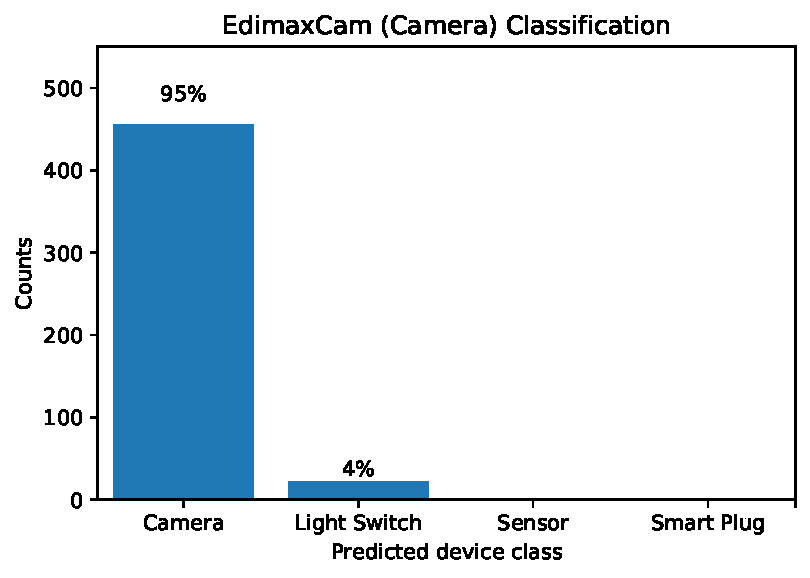
\includegraphics[width=\textwidth]{images/results/iot_clasf_cam_recognition.pdf}
            \label{fig:iot_unseen_camera}
        }
    \end{minipage}%
    \hfill%
    \begin{minipage}[c]{0.49\linewidth}
        \vspace{0pt}
        \centering
        \subfloat[Class prediction of an "unseen" Light Switch]
        {  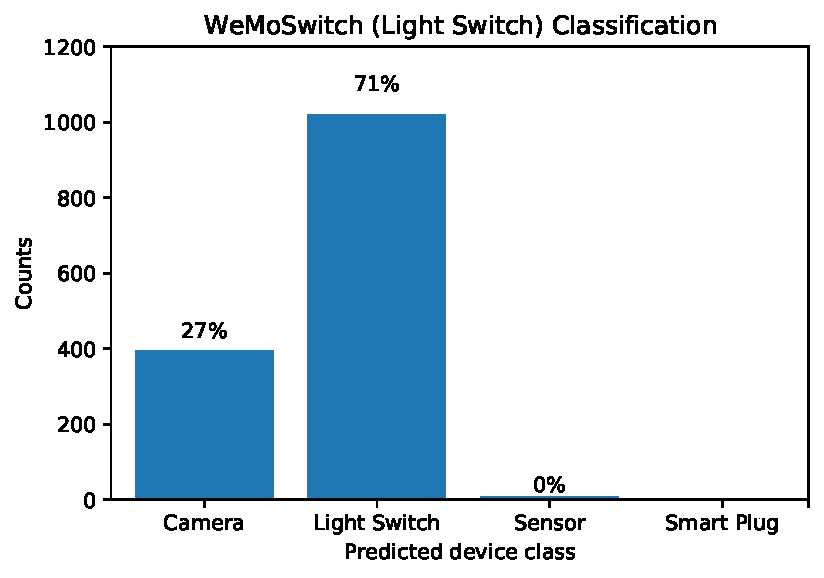
\includegraphics[width=\textwidth]{images/results/iot_clasf_switch_recognition.pdf}
            \label{fig:iot_unseen_light}
        }
    \end{minipage}%
 \caption{Classification of "unseen" device using the trained IoT Sentinel classifiers. Histogram shows the counts of time series assigned to each device class by the classifier. Selected devices belong to the Camera class, shown in \figref{fig:iot_unseen_camera}, and Light Switch class, shown in \figref{fig:iot_unseen_light}; both devices are not included in the dataset shown in \tabref{tab:iotdev}}
 \label{fig:iot_unseen}
\end{figure}

As we can see in all four cases the trained classifiers are able to correctly classify the "unseen" device. It is however important to notice that not all the predictions are done with the same accuracy. More specifically, we can see that, for the devices belonging to the Router and Camera class, more than 95\% time series have been correctly classified. The devices belonging to the PLC and Light Switch class on the other hand, despite being correctly classified, present a non negligible fraction of missclassified time series.

This can be expected since we are considering devices that were not part of the training dataset and the ability alone of the classifier of correctly identifying them is already a great achievement. A more precise classification can be achieved using larger training dataset with more included devices.


\section{Discussion}

In the previous sections we evaluated the performances of the proposed architectures over the two datasets. The results show that the classifiers are able to solve the identification task with great test accuracy. Looking at the loss function and accuracy plot we see a regular behaviour, allowing us to exclude the presence of over or under fitting. This fact, alongside with the overall test accuracy obtained, validates the choice made for the architecture and lookback value in both situations as well as the overall proposed approach.

Looking at the presented confusion matrices we estimated the overall test accuracy, obtaining very high values in both cases. This translates, in a real world application, in the ability, of a trained classifier, of correctly recognizing a device that was included in its training dataset with great precision.

The use of trained classifier to identify devices not included in the training dataset show that the proposed architectures are able to recognize similarities in the device behaviour and, consequently, of correctly classifying them. This result is really important since it demonstrates the capability, of a trained classifier, to easily adapt to new devices and technologies. In a real world application this translates in the possibility of truly implementing this type of classifier as a device identifier, without the necessity of executing a new training procedure whenever newly developed device is connected to the supervised network.